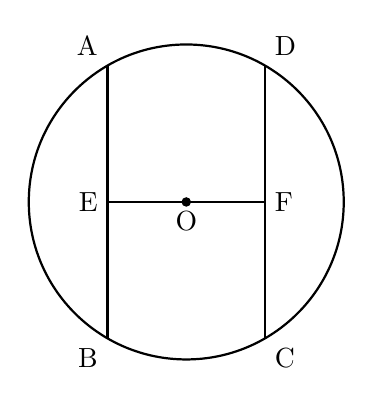
\begin{tikzpicture}[scale=1]

    % Define center of the circle
    \coordinate (O) at (0, 0);

    % Draw the main circle
    \draw[thick] (O) circle (2);

    % Define points for chords AB and CD
    % AB is a vertical chord on the left
    \coordinate (A) at (-1, 1.732);
    \coordinate (B) at (-1, -1.732);
    
    % CD is a vertical chord on the right
    \coordinate (D) at (1, 1.732);
    \coordinate (C) at (1, -1.732);

    % Define points E and F on the chords
    \coordinate (E) at (-1, 0);
    \coordinate (F) at (1, 0);

    % Draw chord AB
    \draw[thick] (A) -- (B);

    % Draw chord CD
    \draw[thick] (C) -- (D);

    % Draw segment EF passing through O
    \draw[thick] (E) -- (F);
    
    % Draw center point O
    \filldraw (O) circle (1.5pt);

    % Add labels
    \node[above left] at (A) {A};
    \node[below left] at (B) {B};
    \node[below right] at (C) {C};
    \node[above right] at (D) {D};
    
    \node[left] at (E) {E};
    \node[right] at (F) {F};
    \node[below] at (O) {O};

\end{tikzpicture}